\documentclass[11pt]{article}
\usepackage[margin=1in]{geometry}
\usepackage{amsmath,amssymb,amsthm}
\usepackage{graphicx}
\usepackage{booktabs}
\usepackage{tabularx}
\usepackage{placeins}
\usepackage{xcolor}
\usepackage[colorlinks=true,linkcolor=blue!45!black,citecolor=green!35!black,
  urlcolor=blue!55!black]{hyperref}

\newtheorem{theorem}{Theorem}[section]
\newtheorem{proposition}[theorem]{Proposition}
\newtheorem{lemma}[theorem]{Lemma}
\newtheorem{corollary}[theorem]{Corollary}
\theoremstyle{definition}
\newtheorem{definition}[theorem]{Definition}
\newtheorem{example}[theorem]{Example}
\theoremstyle{remark}
\newtheorem{remark}[theorem]{Remark}

\newcommand{\F}{\mathbb{F}}
\newcommand{\Z}{\mathbb{Z}}
\newcommand{\ii}{\mathrm{i}}
\newcommand{\Norm}{N}
\newcommand{\Q}{\mathbb{Q}}
\newcommand{\N}{\mathbb{N}}
\newcommand{\PP}{\mathbb{P}}
\newcommand{\R}{\mathbb{R}}
\newcommand{\C}{\mathbb{C}}
\pdfstringdefDisableCommands{\def\F#1{F#1}\def\Z{Z}\def\ii{i}}

\title{\textbf{Finite Trigonometry over \texorpdfstring{$\F_7$}{F7}}\\[0.4em]
\large Angles in \texorpdfstring{$\Z/8$}{Z/8}, the Conic \texorpdfstring{$x^2+y^2=1$}{x^2+y^2=1}, and a First Look at Harmonic Analysis}
\author{Mingli Yuan\\[0.3em]
\small with computational assistance from DeepSeek}
\date{\today}

\begin{document}
\maketitle

\begin{abstract}
Over $\F_7$ the conic $x^2+y^2=1$ has exactly eight points.  They form the
norm-one group of $\F_{49}=\F_7[\ii]/(\ii^2+1)$, a cyclic group of order eight.
Writing $\alpha=2+2\ii$ and $\alpha^k=\cos k+\ii\sin k$ defines a finite
trigonometry with angle group $\Z/8$ and values in $\F_7$.  We prove the
Pythagorean, addition, doubling and periodicity identities, draw the finite unit
circle and the angle group, give the stereographic (half-angle) coordinate, and
draw the discrete waveforms, and compare the finite angle group with the Euclidean angle axioms.  A final section introduces the harmonic layer:
the characters of $\Z/8$, the finite Fourier transform, and the difference
between the $\F_7$-valued trigonometric functions and the $\mathbb C$-valued
characters.  We also explain why the angle measure is discrete and why half-angles need not exist.  This is an algebraic and finite theory; it is not a limit-based
real analysis, and the note says explicitly what is and is not claimed.
\end{abstract}

\tableofcontents

\section{Introduction}

Over the real numbers the functions $\cos\theta$ and $\sin\theta$ are defined by
the unit circle $x^2+y^2=1$ and by angles in $\mathbb R/2\pi\Z$.  Over a finite
field the circle is a finite set, the angle group is finite, and the values are
field elements.  The algebraic identities survive; the limiting and continuity
notions do not.

For $\F_7$ the situation is particularly clean.  The conic
\[
  C:\quad x^2+y^2=1
\]
has exactly $7+1=8$ points, and these points form a cyclic group of order $8$
under the multiplication of the field $\F_{49}$.  This gives a finite analogue
of the circle group, with angle group $\Z/8$, and a finite trigonometry whose
identities are polynomial identities over $\F_7$.  Finite-field trigonometry
has been studied in \cite{FFTrig}; the present note is a concrete geometric
model, with explicit figures and computational checks.

The plan is:
\begin{enumerate}
  \item define the field $\F_{49}$ and the norm-one group, and ask whether the norm induces a metric or a topology (Section~\ref{sec:field});
  \item define $\cos k$ and $\sin k$, and prove the basic identities
        (Sections~\ref{sec:cos-sin}--\ref{sec:addition});
  \item draw the finite unit circle and the angle group
        (Sections~\ref{sec:circle}--\ref{sec:angle-group});
  \item compare the finite angle group with the Euclidean angle axioms
        (Section~\ref{sec:euclid});
  \item give the stereographic/half-angle coordinate (Section~\ref{sec:stereo});
  \item draw the discrete waveforms (Section~\ref{sec:waveforms});
  \item introduce the harmonic layers: finite-field characters in $\F_{49}$ and
        the complex Fourier transform (Section~\ref{sec:fourier});
  \item state what is not claimed and what comes next (Section~\ref{sec:boundary}).
\end{enumerate}

Throughout, $\F_7=\{0,1,\dots,6\}$ with arithmetic modulo $7$; standard
background on finite fields is in \cite{Lidl}.  We refer to \cite{Paper0} and
\cite{Paper1} as Paper~0 and Paper~I.  The element
$\ii$ is a formal square root of $-1$; since $-1$ is not a square in $\F_7$
(the squares are $0,1,2,4$), the ring $\F_7[\ii]/(\ii^2+1)$ is a field with
$49$ elements.

\section{The field \texorpdfstring{$\F_{49}$}{F49} and the norm-one group}
\label{sec:field}

\begin{definition}[Norm and norm-one group]
For $z=x+y\ii\in\F_{49}$ define the norm
\[
  \Norm(z)=z\bar z=(x+y\ii)(x-y\ii)=x^2+y^2\in\F_7 .
\]
Let $G=\{z\in\F_{49}^\times:\Norm(z)=1\}$.
\end{definition}

\begin{proposition}\label{prop:group}
$G$ is a cyclic group of order $8$.
\end{proposition}

\begin{proof}
The norm map $\Norm:\F_{49}^\times\to\F_7^\times$ is a surjective homomorphism
of finite groups (the norm of a generator of $\F_{49}^\times$ generates
$\F_7^\times$).  Hence $|G|=48/6=8$.  A subgroup of the cyclic group
$\F_{49}^\times$ is cyclic, so $G$ is cyclic.
\end{proof}

\begin{proposition}\label{prop:alpha}
Let $\alpha=2+2\ii$.  Then $\alpha$ has order $8$, and $G=\langle\alpha\rangle$.
\end{proposition}

\begin{proof}
We compute
\[
  \alpha^2=4+8\ii+4\ii^2=8\ii=\ii,\qquad
  \alpha^4=\ii^2=-1,\qquad
  \alpha^8=1 .
\]
Since $\alpha^2=\ii\ne1$ and $\alpha^4=-1\ne1$, the order of $\alpha$ is $8$.
It lies in $G$ because $\Norm(\alpha)=2^2+2^2=8=1$, and $G$ has order $8$;
therefore $G=\langle\alpha\rangle$.
\end{proof}

The eight powers are
\[
\begin{array}{c|cccccccc}
k & 0 & 1 & 2 & 3 & 4 & 5 & 6 & 7\\ \hline
\alpha^k & 1 & 2+2\ii & \ii & 5+2\ii & -1 & -2-2\ii & -\ii & 2-2\ii
\end{array}
\]
and their coordinates $(x,y)$ are the eight points
\[
  (1,0),\ (2,2),\ (0,1),\ (5,2),\ (6,0),\ (5,5),\ (0,6),\ (2,5).
\]
They are exactly the solutions of $x^2+y^2=1$ in $\F_7^2$.

\subsection{Does the norm induce a metric or a topology?}
\label{subsec:norm-metric}

The norm takes values in $\F_7$, not in an ordered set.  A metric in the
analytic sense is a function $d$ with values in an ordered set, positive on
distinct points and satisfying the triangle inequality.  The candidate
$d(z,w)=\Norm(z-w)$ fails at the first step: $\F_7$ has no canonical order, so
``$\Norm(z-w)\ge0$'' and ``$\Norm(z-w)<r$'' are not meaningful.  The norm is
anisotropic ($\Norm(z)=0$ iff $z=0$, because $-1$ is a nonsquare), but
anisotropy is nondegeneracy, not a metric.

The only absolute value on $\F_7$ is the trivial one ($|0|=0$, $|x|=1$ for
$x\ne0$).  Composing it with the norm gives $|\Norm(z-w)|\in\{0,1\}$, the
discrete metric; the induced topology is the discrete topology.  The Zariski
topology on the finite set of $\F_7$-points is also discrete.  In this analytic
sense the norm gives no interesting metric or topology.

In the algebraic sense the answer is different and richer.  The norm is a
nondegenerate anisotropic quadratic form; its polar form is the dot product
$u\cdot v$, and its isometry group is the orthogonal group
$\mathrm{O}_2(\F_7)$.  The rotation subgroup is exactly the norm-one group
$G=\mathrm{SO}_2(\F_7)\cong\Z/8$, and the conic $C$ is the unit sphere.  So the
norm does induce a \emph{metric vector space} (a quadratic space) with
orthogonality, isometries and a unit sphere; it does not induce a metric space
in the topological sense.

What the norm does induce geometrically is a stratification.  The fibres are
\[
  \Norm^{-1}(0)=\{0\},\qquad
  \Norm^{-1}(a)\cong C \quad(a\in\F_7^\times),
\]
each nonzero fibre being an $8$-point conic and a $G$-torsor under
$z\mapsto\alpha^k z$.  The six nonzero fibres partition $\F_{49}^\times$;
Figure~\ref{fig:norm} shows them.  This is the finite analogue of polar
coordinates: radius $a\in\F_7^\times$, angle $k\in\Z/8$.  The decomposition is a
torsor decomposition, not a canonical group product: the exact sequence
$1\to\Z/8\to\F_{49}^\times\to\F_7^\times\to1$ does not split as a direct
product (the two orders have gcd $2$), and choosing a base point in each fibre
is a noncanonical section.

The cyclic word metric on $G=\Z/8$ (the one used for the angle group) is not
induced by the norm: the norm is constant $1$ on $G$.  It is induced by the
cyclic order of the angle group.

To obtain a genuine metric and topology from the norm one must lift.  The
unramified extension $\Q_{49}/\Q_7$ has residue field $\F_{49}$; the $7$-adic
absolute value gives a metric on $\Q_{49}$, the field norm
$N_{\Q_{49}/\Q_7}$ is continuous, and the finite norm is its reduction modulo
$7$.  This is the natural bridge from the finite norm to $p$-adic analysis; the
finite field itself only carries the discrete topology.

\begin{figure}[htbp]
\centering
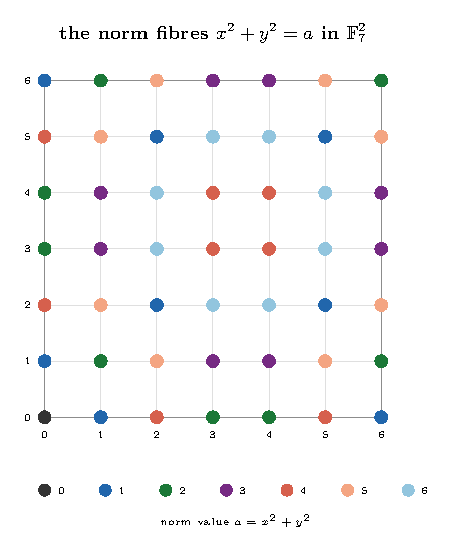
\includegraphics[width=0.56\textwidth]{finite-field-calculi/finite-trig/figures/fig-norm.pdf}
\caption{The norm fibres $x^2+y^2=a$ in $\F_7^2$: the origin ($a=0$) and six
$8$-point conics ($a=1,\dots,6$).  The colours are the norm value; the legend
is at the bottom.  This is a stratification, not a metric topology.}
\label{fig:norm}
\end{figure}

\begin{table}[htbp]
\centering
\small
\begin{tabularx}{\textwidth}{@{}>{\raggedright\arraybackslash}p{0.36\textwidth}X@{}}
\toprule
question & answer\\
\midrule
distance $d(z,w)=\Norm(z-w)$ in an ordered set?
  & no: $\F_7$ is unordered; only the trivial absolute value; discrete topology\\
metric vector space?
  & yes: nondegenerate anisotropic quadratic form; dot product; $\mathrm{O}_2(\F_7)$\\
topology from the norm?
  & discrete; the Zariski topology on the finite points is discrete\\
fibres?
  & $\{0\}$ and six $8$-point conics; $G$-torsors\\
genuine metric or topology?
  & lift to $\Q_{49}/\Q_7$ or $W(\F_{49})$; $7$-adic absolute value\\
metric on $\Z/8$?
  & cyclic word metric, from the group, not from $\Norm$\\
\bottomrule
\end{tabularx}
\caption{What the norm does and does not induce.  The analytic notions
(distance, order, continuity) are absent; the algebraic notions (quadratic
form, isometries, torsors) are present; the analytic version requires a lift.}
\label{tab:norm}
\end{table}

\section{Cos and sin}
\label{sec:cos-sin}

\begin{definition}[Finite cosine and sine]
For $k\in\Z/8$, write
\[
  \alpha^k=\cos k+\ii\,\sin k,\qquad \cos k,\ \sin k\in\F_7 .
\]
\end{definition}

The values are given in Table~\ref{tab:trig}.

\begin{table}[htbp]
\centering
\begin{tabular}{@{}cccc@{}}
\toprule
$k$ & $\alpha^k$ & $\cos k$ & $\sin k$\\
\midrule
0 & $1$       & $1$ & $0$\\
1 & $2+2\ii$  & $2$ & $2$\\
2 & $\ii$     & $0$ & $1$\\
3 & $5+2\ii$  & $5$ & $2$\\
4 & $-1$      & $6$ & $0$\\
5 & $-2-2\ii$ & $5$ & $5$\\
6 & $-\ii$    & $0$ & $6$\\
7 & $2-2\ii$  & $2$ & $5$\\
\bottomrule
\end{tabular}
\caption{The eight angles and their cosines and sines in $\F_7$.}
\label{tab:trig}
\end{table}

\begin{proposition}[Basic identities]\label{prop:basic}
For all $k,l\in\Z/8$:
\begin{enumerate}
  \item (periodicity) $\cos(k+8)=\cos k$ and $\sin(k+8)=\sin k$;
  \item (parity) $\cos(8-k)=\cos k$ and $\sin(8-k)=-\sin k$;
  \item (Pythagoras) $\cos^2 k+\sin^2 k=1$.
\end{enumerate}
\end{proposition}

\begin{proof}
(1) is $\alpha^{k+8}=\alpha^k$.  (2) is $\alpha^{-k}=\overline{\alpha^k}$, using
$\bar\alpha=\alpha^{-1}$.  (3) is $\Norm(\alpha^k)=1$.
\end{proof}

\begin{remark}
The values are in $\F_7$ and the angle is in $\Z/8$; there is no continuous
graph and no real-valued sine wave.  The identities are polynomial identities
in $\F_7$, and they are verified for all $k$ by the script
\texttt{verify.py}.
\end{remark}

\subsection{The angle measure is discrete; there are no radians}
\label{subsec:no-radians}

The protractor is the isomorphism
\[
  \Z/8\longrightarrow G,\qquad k\longmapsto\alpha^k .
\]
The angle is the group element; the label $k$ is its coordinate.  This is the
whole of the finite angle measure.  There is no real-valued additive measure,
no arc length, and no radian: $\F_7$ is unordered, the conic is a finite set,
and there is no continuous arc to length.

One can put a metric on $\Z/8$, the cyclic word metric
\[
  \ell(k)=\min(k,8-k),
\]
but it is a size, not a measure: it is not additive.  For example,
$\ell(3+4)=\ell(7)=1$ while $\ell(3)+\ell(4)=3+4=7$.  The only additive
``measure'' is the group element itself; the word metric is the metric of the
Cayley graph, not a protractor.

The unit is the choice of generator: $\alpha$ generates $G$, and the
automorphisms of $\Z/8$ are multiplication by $1,3,5,7$.  Changing the
generator relabels the eight angles but does not change the group.  The full
turn is $8=0$, the straight angle is $4$, and the right angle is $2$; calling
the generator a ``degree'' is a labelling choice, not a radian.  The periodic
waveforms of Figure~\ref{fig:waveforms} show the period $8$; there is no
interpolation between the eight points.

\section{Addition and doubling}
\label{sec:addition}

\begin{proposition}[Addition formulas]\label{prop:addition}
For all $k,l\in\Z/8$,
\[
  \cos(k+l)=\cos k\cos l-\sin k\sin l,\qquad
  \sin(k+l)=\sin k\cos l+\cos k\sin l .
\]
\end{proposition}

\begin{proof}
Multiply:
\[
  \alpha^{k+l}
  =(\cos k+\ii\sin k)(\cos l+\ii\sin l)
  =(\cos k\cos l-\sin k\sin l)
   +\ii(\sin k\cos l+\cos k\sin l).
\]
The real and imaginary parts are the two displayed identities.
\end{proof}

\begin{corollary}[Doubling]\label{cor:doubling}
For all $k\in\Z/8$,
\[
  \cos 2k=\cos^2 k-\sin^2 k,\qquad
  \sin 2k=2\sin k\cos k .
\]
\end{corollary}

The addition formula is the group law of $\Z/8$ transported to the conic: the
map
\[
  k\longmapsto(\cos k,\sin k)=\alpha^k
\]
is an isomorphism $\Z/8\to G=C(\F_7)$.  The doubling map $k\mapsto2k$ is an
endomorphism of $\Z/8$ with kernel $\{0,4\}$; it is two-to-one, just like the
real doubling map on the circle.  It is \emph{not} an automorphism (the
automorphisms of $\Z/8$ are multiplication by $1,3,5,7$).

\begin{example}
For $k=1$: $\cos1=2$, $\sin1=2$, so $\cos2=4-4=0$ and
$\sin2=2\cdot2\cdot2=8=1$, which is the table entry for $k=2$.
\end{example}

\subsection{Half-angles and division by two}
\label{subsec:half-angle}

The doubling formula gives a map $\Z/8\to\Z/8$, $k\mapsto2k$.  Its kernel is
$\{0,4\}$ and it is two-to-one (Figure~\ref{fig:angle}).  The half-angle
equation is
\[
  2h=k .
\]
It is solvable if and only if $k$ is even; when solvable it has two solutions,
$h$ and $h+4$.  For example, the right angle $k=2$ has $h=1,5$, the straight
angle $k=4$ has $h=2,6$, and the odd angles $k=1,3,5,7$ have no half-angle at
all.

The point is the difference between the field and the angle group:

\begin{itemize}
\item in the field $\F_7$, $2$ is invertible ($2^{-1}=4$), so $2x=a$ has a
      unique solution for every $a$;
\item in the angle group $\Z/8$, $2$ is not invertible, so $2h=k$ may have no
      solution, and when it has one it has two.
\end{itemize}

This is why the half-angle formula for the \emph{square} of the cosine is
well-defined even when the half-angle is not:
\[
  \cos^2 h=\frac{1+\cos k}{2}\qquad(2h=k),
\]
because the right-hand side only uses the field inverse of $2$.  The two
solutions $h$ and $h+4$ give $(\cos h,\sin h)$ and $(-\cos h,-\sin h)$; the
half-angle is defined only up to sign.

Table~\ref{tab:half-angle} summarizes the two equations.  The consequences
are:

\begin{itemize}
\item there is no global half-angle function $\Z/8\to\Z/8$;
\item there is no global angle bisector (the bisector exists only for even $k$,
      and then it is a line with two orientations);
\item the inscribed-angle theorem has only a two-to-one shadow
      (Section~\ref{sec:euclid});
\item the stereographic coordinate $t$ (the slope from $P_0$, the finite
      analogue of $\tan(k/2)$) is a rational coordinate on the seven angles
      $k\ne4$, not a group homomorphism.
\end{itemize}

In Euclidean geometry the angle group $\mathbb R/2\pi\mathbb Z$ is divisible:
$2h=k$ always has two solutions, $h$ and $h+\pi$.  The finite group $\Z/8$ is
not two-divisible, and the failure is not a technicality: it is the absence of
division in $\Z/8$.

\begin{table}[htbp]
\centering
\small
\begin{tabular}{@{}lll@{}}
\toprule
equation & in the field $\F_7$ & in the angle group $\Z/8$\\
\midrule
$2x=a$ & unique solution $x=a/2$ & $2$ if $a$ even; $0$ if $a$ odd\\
half-angle $2h=k$ & unique $h=k/2$ & $2$ if $k$ even; $0$ if $k$ odd\\
\bottomrule
\end{tabular}
\caption{The field inverse of $2$ and the angle equation $2h=k$.  The field has
$2^{-1}=4$; the group $\Z/8$ has no division by $2$.}
\label{tab:half-angle}
\end{table}

\section{The finite unit circle}
\label{sec:circle}

\begin{figure}[htbp]
\centering
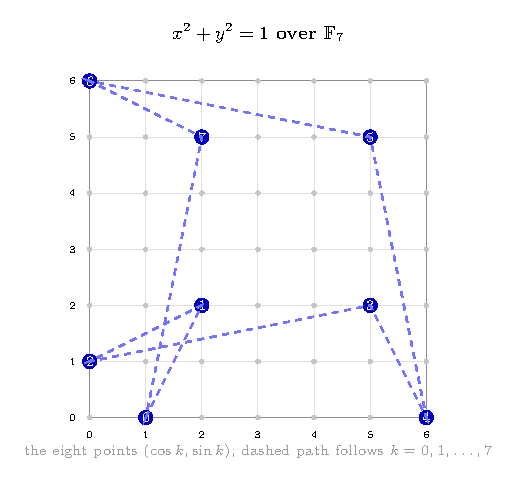
\includegraphics[width=0.52\textwidth]{finite-field-calculi/finite-trig/figures/fig-circle.pdf}
\caption{The eight points of $x^2+y^2=1$ over $\F_7$, labelled by the angle
$k\in\Z/8$.  The dashed path follows $k=0,1,\dots,7$.  This is a conic, not a
Euclidean circle: the eight points are scattered in the $7\times7$ grid.}
\label{fig:circle}
\end{figure}

The conic $C$ is isomorphic to the projective line $\mathbb P^1(\F_7)$; the
eight points of $C(\F_7)$ are the eight points of $\mathbb P^1(\F_7)$.  The
angle $k$ is one coordinate on this set; the stereographic coordinate $t$ of
Section~\ref{sec:stereo} is another.  Neither coordinate is more intrinsic than
the other: the intrinsic object is the conic together with its group law.

\subsection{Centre, angle group, and order}
\label{subsec:center}

\paragraph{Does a centre exist?}
Homogenize the conic as $C:x^2+y^2=z^2$ and let $L_\infty:z=0$.  The polar of
$[a:b:c]$ is $a x+b y-c z=0$, so the pole of $L_\infty$ is
$O=[0:0:1]=(0,0)$.  The point $O$ is not on $C$ ($0\ne1$); it is the unique
point with $\Norm(O)=0$, while every point of $C$ has norm $1$.  The central
symmetry $\sigma(x,y)=(-x,-y)$ preserves $C$ and fixes $O$; on the angle group
it is $\alpha^4$, the half-turn, and it pairs the eight points into four
antipodal pairs $\{k,k+4\}$ (Figure~\ref{fig:center}).

\begin{figure}[htbp]
\centering
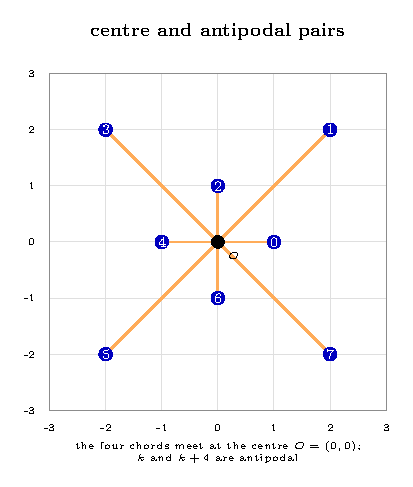
\includegraphics[width=0.46\textwidth]{finite-field-calculi/finite-trig/figures/fig-center.pdf}
\caption{The centre $O=(0,0)$ is the pole of $L_\infty$.  The four chords
through $O$ join the antipodal pairs $k$ and $k+4$.  The centre is not on the
conic.}
\label{fig:center}
\end{figure}

The centre is finite exactly when $L_\infty$ is not tangent to $C$: the ellipse
and the hyperbola have a finite centre, while the parabola's centre is the
tangency point at infinity.

\paragraph{The angle group around the centre.}
The symmetries of $C$ fixing $O$ are the orthogonal group
$\mathrm{O}_2(\F_7)$ of the quadratic form $x^2+y^2$, a dihedral group of
order $16$.  Its rotation subgroup is
\[
  G=\mathrm{SO}_2(\F_7)\cong\Z/8,
\]
the norm-one group; it acts regularly on $C$.  The angle of a point $P$ relative
to a base point $P_0$ is the unique $k\in\Z/8$ with $P=\alpha^k P_0$; the
rotations are the angle group around the centre.

The full conic automorphism group is $\mathrm{PGL}_2(7)$ of order $336$.  It
does not fix $O$: the stabilizer of $O$ is $\mathrm{O}_2(\F_7)$ of order $16$,
so the orbit of $O$ has $336/16=21$ points, the internal points of the
polarity.  Thus the centre is extra structure: the conic alone is
$\mathbb P^1$ with $\mathrm{PGL}_2(7)$; a centre (equivalently a line at
infinity) selects the angle group.  This is the same point as the earlier
frame discussion: the ``circle'' is not just the conic.

\paragraph{Order: cyclic, not total.}
The angle group $\Z/8$ is cyclic; a generator $\alpha$ gives a cyclic order
\[
  0,1,2,\dots,7
\]
on $C$.  The rotations preserve this cyclic order, the reflections in
$\mathrm{O}_2(\F_7)$ reverse it, and the full symmetry of the cyclic order is
the dihedral group $\mathrm{O}_2(\F_7)$ of order $16$.

There is no \emph{total} order invariant under the rotations.  An
order-preserving permutation of a finite chain is the identity (the least
element must be fixed, then inductively all the others), whereas the rotation
by one step is an $8$-cycle.  One can choose a total order by cutting the circle
at a base point and declaring $0<1<\dots<7$, but the cut depends on the base
point and is moved by the rotations; it is not canonical.

This is the finite analogue of the Euclidean circle.  The circle has a
\emph{cyclic} order (an orientation), not a linear order; the real line has a
linear order, the circle does not.  The angle $k$ is a coordinate on the cyclic
order, not a linear order.  The cyclic betweenness is also different from the
linear one: for any three points, one lies on the oriented arc from one of the
others to the third; this relation is preserved by rotations and reversed by
reflections.

\begin{table}[htbp]
\centering
\small
\begin{tabularx}{\textwidth}{@{}>{\raggedright\arraybackslash}p{0.13\textwidth}>{\raggedright\arraybackslash}p{0.13\textwidth}>{\raggedright\arraybackslash}p{0.24\textwidth}>{\raggedright\arraybackslash}p{0.10\textwidth}X@{}}
\toprule
model & centre & affine stabiliser & angle group & cyclic order\\
\midrule
ellipse & $(0,0)$ & $\mathrm{O}_2(\F_7)\cong D_8$ & $\Z/8$ & $8$ points\\
hyperbola & $(0,0)$ & $\mathrm{O}_{1,1}(\F_7)\cong D_6$ & $\Z/6$ & $6$ finite $+$ $2$ fixed\\
parabola & at infinity & $\mathrm{AGL}_1(\F_7)$ & $\Z/7$ & $7$ finite $+$ $1$ fixed\\
\bottomrule
\end{tabularx}
\caption{The centre, the affine stabiliser, and the regular angle group for the
three models.  The centre is finite iff $L_\infty$ is not tangent; the order of
the regular angle group is $q+1$, $q-1$, $q$ for the ellipse, hyperbola and
parabola.}
\label{tab:center}
\end{table}

Table~\ref{tab:center} records the three models.  The regular angle group is
the subgroup acting regularly on the finite points: for the ellipse and
hyperbola it is the rotation part of the affine stabiliser, while for the
parabola it is the unipotent part.  The parabola's full affine stabiliser is
$\mathrm{AGL}_1(\F_7)$ of order $42$, not the dihedral group $D_7$ of order $14$;
$D_7$ is only the subgroup with linear part $a=\pm1$.  The points fixed by the
regular action are the intersections of $L_\infty$ with $C$ (none for the
ellipse, two for the hyperbola, one for the parabola).

\subsection{Arcs, gluing, and transitivity}
\label{subsec:arcs}

A directed arc is an interval of the cyclic order.  Write $[a,b]_\ell$ for the
arc that starts at $a$ and has length $\ell\in\{0,1,\dots,8\}$; its point set is
$\{a,a+1,\dots,a+\ell\}$ modulo $8$.  The length $\ell$ is the angle difference
$b-a$; $\ell=0$ is the point $a$, and $\ell=8$ is the full circle.

Gluing two arcs is defined when the endpoint of the first is the start of the
second:
\[
  [a,b]_\ell\cdot[b,c]_m=[a,c]_{\ell+m}
  \qquad(\ell+m\le8).
\]
If $\ell+m>8$ the composite wraps more than once and is no longer a simple arc.
Thus the simple arcs form a \emph{partial} monoid, not a monoid.  If one keeps
the winding, i.e.\ lets the length be an integer in $\Z$ and records the
projection $b-a\equiv\ell\pmod8$, the arcs form the action groupoid of $\Z$ on
$\Z/8$: objects are the eight points, arrows are the based arcs, composition is
gluing, and the automorphism group of a point is $\Z$ (the full turns).  If only
nonnegative lengths are allowed, one gets the action category of $\N$; the
endomorphism monoid of a point is $\N$ (full turns), not a group.

The question of transitivity has three different answers.

\begin{enumerate}
\item \emph{The one-step relation.}  For a nonempty set $S\subseteq\Z/8$ of
      allowed lengths, let $a\,R_S\,b$ iff $b-a\in S$.  Then $R_S$ is
      transitive if and only if $S$ is a subgroup of $\Z/8$.  The subgroups are
      \[
        \{0\},\qquad \{0,4\},\qquad \{0,2,4,6\},\qquad \Z/8,
      \]
      with $8,4,2,1$ classes respectively: equality, antipodal pairs, parity,
      and the universal relation.
\item \emph{Reachability.}  The relation $R_S^*$ (a finite sequence of allowed
      steps) is transitive by construction.  Its classes are the cosets of the
      subgroup $\langle S\rangle$ generated by $S$; the number of components is
      \[
        [\Z/8:\langle S\rangle].
      \]
      The reachability graph has one component exactly when
      $\langle S\rangle=\Z/8$; the reachability relation itself is always
      transitive.
\item \emph{The arc category.}  With all lengths allowed, the arc groupoid is
      transitive (connected): any point reaches any other point.  With a
      restricted set $S$ of lengths, one gets the subgroupoid of
      $\langle S\rangle$; it is transitive on each coset, not on the whole
      circle unless $S$ generates $\Z/8$.
\end{enumerate}

Figure~\ref{fig:arcs} shows the first three steps.  Table~\ref{tab:arcs}
records the components and the one-step transitivity for representative sets.

\begin{figure}[htbp]
\centering
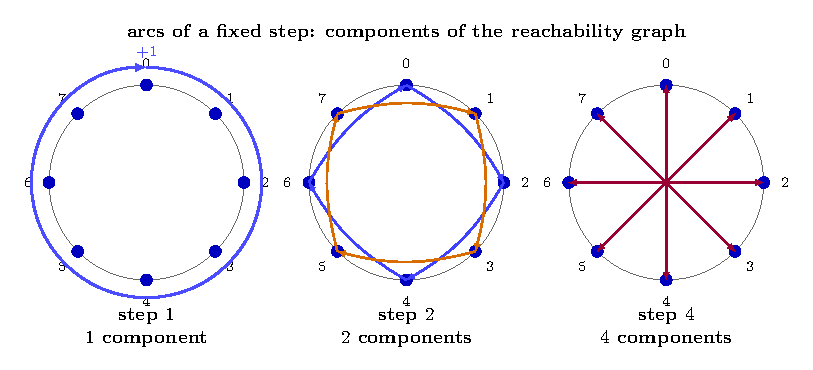
\includegraphics[width=0.86\textwidth]{finite-field-calculi/finite-trig/figures/fig-arcs.pdf}
\caption{Arcs of a fixed step $k$: the components of the reachability graph.
$k=1$ gives one $8$-cycle; $k=2$ gives two $4$-cycles (parity); $k=4$ gives four
$2$-cycles (antipodal pairs).}
\label{fig:arcs}
\end{figure}

\begin{table}[htbp]
\centering
\small
\begin{tabular}{@{}llll@{}}
\toprule
$S$ & $\langle S\rangle$ & components & $R_S$ transitive?\\
\midrule
$\{1\}$ & $\Z/8$ & $1$ & no\\
$\{2\}$ & $\{0,2,4,6\}$ & $2$ (parity) & no\\
$\{3\}$ & $\Z/8$ & $1$ & no\\
$\{4\}$ & $\{0,4\}$ & $4$ (antipodal) & no\\
$\{2,4\}$ & $\{0,2,4,6\}$ & $2$ & no\\
$\{0,4\}$ & $\{0,4\}$ & $4$ & yes\\
$\Z/8$ & $\Z/8$ & $1$ & yes\\
\bottomrule
\end{tabular}
\caption{Allowed arc lengths $S$, the subgroup they generate, the number of
reachability components, and whether the one-step relation is transitive.  For
nonempty $S$ the one-step relation is transitive exactly for the subgroups;
reachability is always transitive, and it has exactly one component when $S$
generates $\Z/8$.}
\label{tab:arcs}
\end{table}

The figure and the table make the point precise.  The full arc structure is
transitive, but a restricted arc structure need not be: the arcs of step $2$
never connect an even point to an odd one, and the arcs of step $4$ only
connect antipodal pairs.  The components are always the cosets of
$\langle S\rangle$.

This is the finite analogue of the fundamental groupoid of the circle.  The
topological circle has path groupoid with automorphism group
$\pi_1(S^1)=\Z$; the finite arc groupoid with winding has the same automorphism
group $\Z$, and its projection to the eight points is the quotient by the full
turn $8$.  The simple arcs form a partial composition structure (composition is defined
only when the total length is at most $8$); the action groupoid of $\Z$
(integer winding) is the groupoid with automorphism group $\Z$.  Calling the
simple arcs a ``fundamental category'' is only informal; the categorical
structure with integer winding is the groupoid.

\subsection{Experiment: translating the circle}
\label{subsec:translate}

Translate every point of $C$ by one cell upward:
\[
  T(x,y)=(x,y+1).
\]
The image of the conic is
\[
  C':\quad x^2+(y-1)^2=1,
\]
with the eight points
\[
  (1,1),\ (2,3),\ (0,2),\ (5,3),\ (6,1),\ (5,6),\ (0,0),\ (2,6).
\]

The unit-circle relation is \emph{not} preserved: none of the new points has
norm $1$ with respect to the original norm.  Their norms are
\[
  2,\ 6,\ 4,\ 6,\ 2,\ 5,\ 0,\ 5,
\]
so the new set is not the norm-one fibre of $N(x,y)=x^2+y^2$.  The centre moves
from $O=(0,0)$ to $O'=T(O)=(0,1)$.  The two centres exchange roles: the old
centre $O$ lies on $C'$ because $0+(0-1)^2=1$, and the new centre $O'$ lies on
$C$ because $0+1^2=1$.  The two conics are disjoint: $C\cap C'$ would require
\[
  y^2=(y-1)^2\ \Longrightarrow\ 2y=1\ \Longrightarrow\ y=4,
  \qquad x^2+16=x^2+2=1\ \Longrightarrow\ x^2=6,
\]
and $6$ is a nonsquare in $\F_7$.

The image is nevertheless \emph{still a conic}.  The reason is that $T$ is an
affine transformation, and affine transformations preserve conics.  In fact $T$
fixes $L_\infty$ pointwise, so $C'$ is again an ellipse; the angle group is the
conjugate
\[
  T\,G\,T^{-1}\cong\Z/8,
\]
which fixes $O'$ and acts regularly on $C'$.  The cyclic order and the arc
structure are transported by $T$; transitivity is unchanged.

\begin{figure}[htbp]
\centering
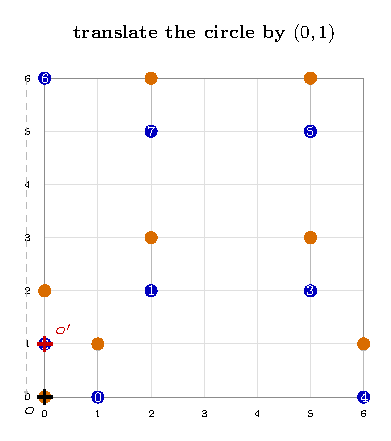
\includegraphics[width=0.58\textwidth]{finite-field-calculi/finite-trig/figures/fig-translate.pdf}
\caption{The original conic (blue, $x^2+y^2=1$) and its translate (orange,
$x^2+(y-1)^2=1$) under $(x,y)\mapsto(x,y+1)$.  The two conics are disjoint; the
old centre $O=(0,0)$ is a point of the orange conic, and the new centre
$O'=(0,1)$ is a point of the blue one.}
\label{fig:translate}
\end{figure}

\begin{table}[htbp]
\centering
\small
\begin{tabular}{@{}lll@{}}
\toprule
 & original $C$ & translated $C'$\\
\midrule
equation & $x^2+y^2=1$ & $x^2+(y-1)^2=1$\\
centre & $(0,0)$ & $(0,1)$\\
norm $N(x,y)=x^2+y^2$ & constant $1$ & $0,2,4,5,6$\\
$L_\infty$ & disjoint & disjoint\\
angle group & $G$ & $TGT^{-1}\cong\Z/8$\\
\bottomrule
\end{tabular}
\caption{The unit circle and its translate.  The conic property and the
projective/affine structure survive; the centre and the norm-one relation do
not.}
\label{tab:translate}
\end{table}

The moral is the distinction between the projective and the affine data.  A
conic is preserved by every projectivity, in particular by every translation;
the unit-circle data --- the centre $O$, the norm $N$, and the angle group
around $O$ --- are not.  A uniform translation gives another conic (a circle
with a new centre), not the same circle.  If the eight points were moved by an
arbitrary permutation instead of a translation, the image would generally not
be a conic at all; the conic property is projective/affine-invariant, not
permutation-invariant.

\subsection{Movable circles and transportability}
\label{subsec:movable}

The right definition is not a fixed subset but a relative relation.  For a centre
$O$ and a radius parameter $r\in\F_7$, put
\[
  S(O,r)=\{P:Q(P-O)=r\},\qquad Q(v)=v_1^2+v_2^2 .
\]
The unit circle is $S(0,1)$; the translated circle of the previous experiment is
$S((0,1),1)$.  The relation is translation-equivariant:
\[
  T\bigl(S(O,r)\bigr)=S\bigl(T(O),r\bigr)
\]
for every translation $T$.  The absolute norm $N(P)=Q(P)$ is not
translation-invariant; the relative norm $Q(P-O)$ is.  That is the movable
circle relation.  In Euclidean language $r$ is the square of the radius; over
$\F_7$ the square root need not exist, so $r$ is the honest parameter.

The family of circles is
\[
  \mathcal C=\{(O,r):O\in\F_7^2,\ r\in\F_7\}.
\]
The translations act transitively on the centres with $r$ fixed.  For the
linear part there are three different groups, and they must not be conflated:
\begin{itemize}
  \item the orthogonal group $\mathrm O(Q)$: $Q(Av)=Q(v)$;
  \item the scalar similarities $\F_7^\times\mathrm O(Q)$: $A=\lambda R$,
        $Q(Av)=\lambda^2Q(v)$;
  \item the full similarity group $\mathrm{GO}(Q)$: $Q(Av)=\mu Q(v)$ for some
        $\mu\in\F_7^\times$.
\end{itemize}
General quadratic-form theory uses the last group.  Its elements need not be
scalar multiples of orthogonal maps: for example
\[
  A=\begin{pmatrix}1&4\\3&1\end{pmatrix},
  \qquad A^{T}A=3I,
\]
so $Q(Av)=3Q(v)$ and $A(S_1)=S_3$, although $3$ is a nonsquare in $\F_7$.

\begin{table}[htbp]
\centering
\small
\begin{tabular}{@{}llll@{}}
\toprule
group & definition & order & orbits on nonzero $S_r$\\
\midrule
$\mathrm O(Q)$ & $Q(Av)=Q(v)$ & $16$ & six\\
$\F_7^\times\mathrm O(Q)$ & $A=\lambda R$ & $48$ & two square classes\\
$\mathrm{GO}(Q)$ & $Q(Av)=\mu Q(v)$ & $96$ & one\\
\bottomrule
\end{tabular}
\caption{The three linear groups.  $\mathrm{GO}(Q)$ is the full similarity
group of the quadratic form; the scalar similarities are the subgroup with
$\mu$ a square.  The orbit counts on the six nonzero norm circles are
$6$, $2$, and $1$.}
\label{tab:similarity-groups}
\end{table}

\begin{table}[htbp]
\centering
\small
\begin{tabular}{@{}lll@{}}
\toprule
group & action on $(O,r)$ & preserves circles?\\
\midrule
translations & $O\mapsto O+t$, $r$ fixed & yes\\
$\F_7^\times\mathrm O(Q)$ & $O\mapsto\lambda RO+t$, $r\mapsto\lambda^2r$ & yes\\
$\mathrm{GO}(Q)$ & $O\mapsto AO+t$, $r\mapsto\mu r$ & yes\\
affine & $O\mapsto AO+t$ & iff $A\in\mathrm{GO}(Q)$; otherwise ellipses\\
projective & general & iff $\{I,J\}$ is preserved; otherwise conics\\
\bottomrule
\end{tabular}
\caption{The circle is a similarity structure, not merely an affine or
projective one.  The full similarity group $\mathrm{GO}(Q)$ acts transitively on
the nonzero circles; the scalar similarities $\F_7^\times\mathrm O(Q)$ have the
two square-class orbits.  $I,J$ are the circular points at infinity.}
\label{tab:circles}
\end{table}

The circular points make the distinction precise.  Homogenize
$Q(x,y)=x^2+y^2$ and put $z=0$: the two points
\[
  I=[1:\ii:0],\qquad J=[1:-\ii:0]
\]
in $\PP^2(\F_{49})$ satisfy $x^2+y^2=0$.  A conic is a circle exactly when it
passes through $I$ and $J$.  The stabilizer of the pair $\{I,J\}$ in the
projective group is the full affine similarity group $\mathrm{GO}(Q)$; a
general affine map acts on the line at infinity by its linear part and moves
$I,J$ unless the linear part lies in $\mathrm{GO}(Q)$, so it sends a circle to
an ellipse; a general projectivity sends a circle to a conic not through $I,J$.
The conic is projective; the circle is a similarity notion.

The angle group is transported with the centre and the circle.  The stabilizer
of $O$ \emph{and} a nonzero circle $S_r$ in the affine similarity group is
$\mathrm O(Q)$; its rotation subgroup is $G=\mathrm{SO}(Q)\cong\Z/8$.  For the
translated circle the angle group is $TGT^{-1}$, and the cyclic order and the
arc structure are transported by $T$.  The stabilizer of $O$ alone is the
larger group $\mathrm{GO}(Q)$: it also contains the dilations that move the
circle, and those are not angle rotations.  Thus the whole rigid structure ---
centre, a chosen circle, angle group, cyclic order, arcs --- is transportable
under translations, and under the full similarity group up to the choice of the
radius.

The square classes are the obstruction for the \emph{scalar} similarities
$\F_7^\times\mathrm O(Q)$, not for $\mathrm{GO}(Q)$:
\[
  \F_7^\times/\F_7^{\times2}=\{\{1,2,4\},\{3,5,6\}\}.
\]
Under $\F_7^\times\mathrm O(Q)$ the unit circle is similar only to the
square-radius circles.  Under $\mathrm{GO}(Q)$ it is similar to every nonzero
circle, because the multiplier $\mu$ may be a nonsquare.  Over $\R$ the
positive scalar similarities already act transitively on the positive radii;
over $\F_7$ the scalar multipliers are squares, hence the two orbits, and
$\mathrm{GO}(Q)$ adds the nonsquare multipliers that repair the gap.

\subsection{Scaling and the ripple pencil}
\label{subsec:ripple}

There are two different families of circles attached to the centre $0$, and the
scaling group acts on them differently.

\paragraph{The norm circles.}
The level sets
\[
  S_r=\{P:Q(P)=r\},\qquad r\in\F_7^\times,
\]
are the six $8$-point conics centred at $0$; $S_0=\{0\}$.  The dilation
$D_\lambda(P)=\lambda P$ acts by
\[
  D_\lambda(S_r)=S_{\lambda^2r}.
\]
Since $\lambda^2$ runs over the squares $\{1,2,4\}$, the six circles split into
two scaling orbits,
\[
  \{S_1,S_2,S_4\},\qquad \{S_3,S_5,S_6\},
\]
the square classes of the radius.

\paragraph{The ripple pencil.}
The affine clue horocycles in the finite model are the horizontal lines
\[
  H_t=\{x+ti:x\in\F_7\},\qquad t\in\F_7 ,
\]
with seven points each.  In the projective line
$\PP^1(\F_{49})=\F_{49}\cup\{\infty\}$ put
$\widehat H_t=H_t\cup\{\infty\}$.  The M\"obius inversion
\[
  J(z)=-\frac1z
\]
acts on $\PP^1(\F_{49})$ and maps
\[
  J(\widehat H_t)=C_t:\quad x^2+y^2=\frac{y}{t},
  \qquad t\in\F_7^\times .
\]
Equivalently, on affine points, $J(H_t)=C_t\setminus\{0\}$: the missing point
is exactly the pole $0=J(\infty)$.  Every $C_t$ is an $8$-point conic through
$0$, and all six share the tangent line $y=0$ at $0$.  They form the finite
\emph{ripple pencil}.  The correspondence
\[
  J(\widehat H_t)=C_t
\]
is exact: the point path (the clue) and the ripple history are two readings of
the same M\"obius map, as in the path--ripple duality of Paper~0.

Three spaces must be kept apart: the affine plane $\mathbb A^2(\F_7)$ has
$49$ points; the projective plane $\PP^2(\F_7)$ has $57$; the M\"obius line
$\PP^1(\F_{49})$ has $50$.  The infinity in $\widehat H_t$ is the one of
$\PP^1(\F_{49})$, not a line at infinity of $\PP^2(\F_7)$.

Under the same dilation, the ripple parameter transforms by
\[
  D_\lambda(C_t)=C_{t/\lambda}.
\]
Here $\lambda$ runs over all of $\F_7^\times$, not just the squares, so the six
ripple conics form a \emph{single} orbit
\[
  \{C_1,C_2,\dots,C_6\}.
\]
This is the precise finite form of the nested family of Euclidean circles
tangent at $0$: the nesting parameter $t$ is the height of the clue line, and
the scaling acts on it by the inverse scalar $\lambda^{-1}$.

\begin{figure}[htbp]
\centering
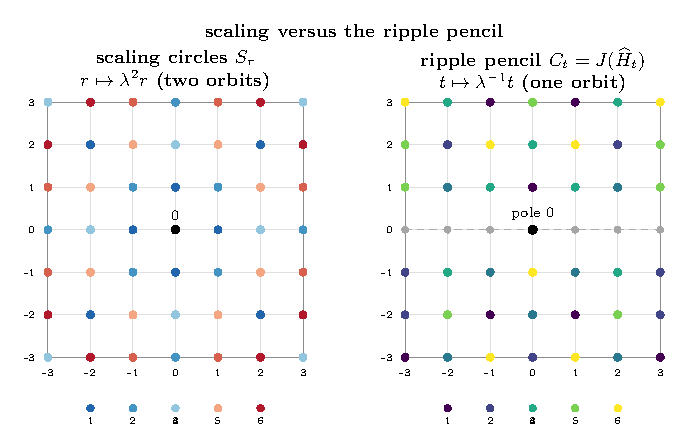
\includegraphics[width=0.88\textwidth]{finite-field-calculi/finite-trig/figures/fig-ripple.pdf}
\caption{Left: the norm circles $S_r$ (level sets of $Q$), coloured by $r$;
their scaling orbits are the two square classes.  Right: the ripple conics
$C_t=J(\widehat H_t)$, all through the pole $0$ with common tangent $y=0$; the grey points on the $x$-axis are the
clue line $H_0$.  In the Euclidean upper half-plane the $C_t$ are nested circles
tangent at $0$; over $\F_7$ they form a pencil of six $8$-point conics through
$0$.}
\label{fig:ripple}
\end{figure}

\begin{table}[htbp]
\centering
\small
\begin{tabular}{@{}lllll@{}}
\toprule
family & equation & common point & scaling & orbits\\
\midrule
clue lines $H_t$ & $y=t$ & $\infty$ & $t\mapsto\lambda t$ & one\\
ripple conics $C_t$ & $x^2+y^2=y/t$ & $0$ & $t\mapsto\lambda^{-1}t$ & one\\
norm circles $S_r$ & $x^2+y^2=r$ & none & $r\mapsto\lambda^2r$ & two square classes\\
\bottomrule
\end{tabular}
\caption{The clue lines $H_t$ and the ripple conics $C_t=J(\widehat H_t)$ are exchanged by
the inversion $J(z)=-1/z$; scaling acts by the inverse scalar on $t$.  The
orbit counts are for nonzero $t$ and $r$; $t=0$ (the $x$-axis) and $r=0$ (the
origin) are fixed.  The norm circles $S_r$ are a different family, with the
square-class obstruction for scalar similarities.}
\label{tab:ripple}
\end{table}

The visual point is worth stating plainly.  The Euclidean picture of the ripple
family is a nested family of circles tangent at $0$; the nesting is an ordered
notion (inside/outside, radius).  Over $\F_7$ there is no such order: the six
$C_t$ are $8$-point conics through $0$, and their arrangement on the $7\times7$
grid is a coloured partition, not a sequence of nested rings.  What is
observable is the \emph{pencil} (all six through the pole), the \emph{partition}
of the grid, and the scaling action; what is not observable is the Euclidean
nesting.  The correspondence $J(\widehat H_t)=C_t$ and the scaling laws
$t\mapsto\lambda^{-1}t$, $r\mapsto\lambda^2r$ hold exactly; they are algebraic
statements, not visual ones.

\subsection{The real picture and the finite picture}
\label{subsec:real-finite}

It is worth placing the finite ripple pencil next to the real one from
Paper~0.  Over $\R$, with $J(z)=-1/z$ and the affine line
$H_t=\{x+ti:x\in\R\}$, $t>0$, put $\widehat H_t=H_t\cup\{\infty\}$ in the
Riemann sphere $\PP^1(\C)$.  The image is the circle
\[
  C_t:\quad x^2+\Bigl(y-\frac1{2t}\Bigr)^2=\Bigl(\frac1{2t}\Bigr)^2,
  \qquad t>0 .
\]
All these circles are tangent to the real axis at $0$ and nested as $t$ varies;
the parameter $t$ is continuous.  The compactified clue lines and the circles
are exchanged by $J$:
\[
  J(\widehat H_t)=C_t .
\]
On affine points $J(H_t)=C_t\setminus\{0\}$; the missing point is the pole
$0=J(\infty)$.  The dilation $D_\lambda$, $\lambda>0$, sends $t$ to
$t/\lambda$; the family is a single orbit, and the nesting is visible.

Over $\F_7$ the same equations produce the six conics
\[
  C_t:\quad x^2+y^2=\frac{y}{t},\qquad t\in\F_7^\times .
\]
They all pass through the pole $0$ with the common tangent $y=0$, and they form
a \emph{pencil}, not a nested sequence.  The correspondence
$J(\widehat H_t)=C_t$ and the scaling law $t\mapsto t/\lambda$ still hold; the
six form one orbit.  What is lost is the order: there is no inside/outside, no
continuous parameter, no nesting.

\begin{figure}[htbp]
\centering
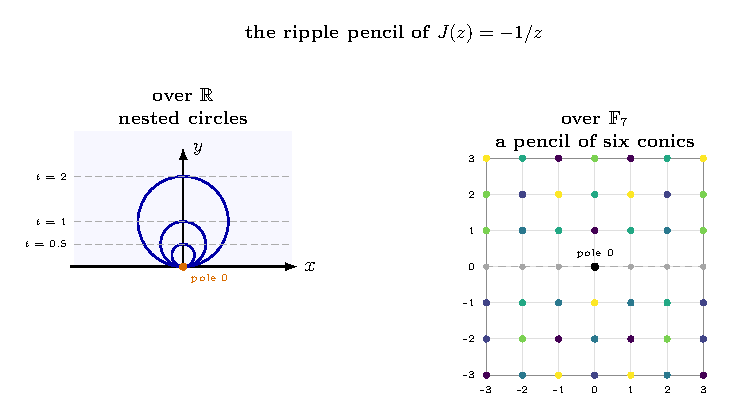
\includegraphics[width=0.92\textwidth]{finite-field-calculi/finite-trig/figures/fig-ripple-compare.pdf}
\caption{The ripple pencil of $J(z)=-1/z$ over $\R$ and over $\F_7$.  Left: the
compactified clue lines $\widehat H_t$ (dashed affine part $H_t$ plus $\infty$)
map to nested circles tangent at $0$; the affine part misses the pole $0$.
Right: the same equations over $\F_7$ give six $8$-point conics through $0$,
with common tangent $y=0$; the family is a pencil, not a nested sequence.}
\label{fig:compare}
\end{figure}

\begin{table}[htbp]
\centering
\small
\begin{tabular}{@{}lll@{}}
\toprule
 & over $\R$ & over $\F_7$\\
\midrule
parameter & $t>0$ continuous & $t\in\F_7^\times$ (six values)\\
$C_t$ & nested circles tangent at $0$ & $8$-point conics through $0$, common tangent $y=0$\\
ordering & nesting by $t$ & no order; pencil\\
scaling & $t\mapsto t/\lambda$, $\lambda>0$ & $t\mapsto t/\lambda$, $\lambda\in\F_7^\times$\\
orbits & one & one\\
$J(\widehat H_t)=C_t$ & yes & yes\\
visual & nested rings & coloured pencil\\
\bottomrule
\end{tabular}
\caption{The real and finite ripple pencils.  The algebraic correspondence and
the scaling orbit are field-independent; the nesting is a real/order
phenomenon.}
\label{tab:compare}
\end{table}

The moral is the same one that has recurred throughout these notes: the
\emph{algebraic} structure --- the conic family, the M\"obius correspondence, the
scaling orbit --- is field-independent, while the \emph{order} structure ---
nesting, inside/outside, continuous parameter --- is special to $\R$.  The
finite ``ripple geometry'' is a pencil, not a new geometry; the name is
descriptive, as Paper~0 says of its real counterpart.

\section{The angle group}
\label{sec:angle-group}

\begin{figure}[htbp]
\centering
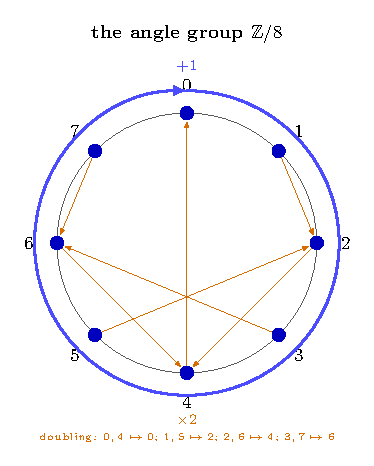
\includegraphics[width=0.42\textwidth]{finite-field-calculi/finite-trig/figures/fig-angle-cycle.pdf}
\caption{The angle group $\Z/8$.  The blue outer arrow is the $+1$ cycle; the
orange chords are the doubling map $k\mapsto2k$.  Doubling is two-to-one:
$0,4\mapsto0$; $1,5\mapsto2$; $2,6\mapsto4$; $3,7\mapsto6$.}
\label{fig:angle}
\end{figure}

The angle group is the cyclic group $\Z/8$.  Its automorphism group is
$(\Z/8)^\times=\{1,3,5,7\}$; multiplication by $3,5,7$ permutes the eight angles,
while multiplication by $2$ collapses pairs.  The addition formula of
Proposition~\ref{prop:addition} is the statement that the conic's group law and
the angle group's addition are the same operation.

\FloatBarrier
\section{Euclidean angle axioms and the finite angle group}
\label{sec:euclid}

There are two different finite analogues of a Euclidean angle, and they must be
kept apart:
\begin{itemize}
  \item the \emph{unit-vector angle} between two points of the conic
        $C:x^2+y^2=1$, with values in $G=\Z/8$;
  \item the \emph{line-direction angle} between two lines through the origin,
        with values in $D=\F_{49}^\times/\F_7^\times$, also isomorphic to
        $\Z/8$.
\end{itemize}
The first is a point-on-conic coordinate; the second is a direction ratio.  The
unit circle meets only four of the eight lines through the origin, each in a
pair of antipodal points, so the unit-vector angle does not cover all
directions.  That is not a failure of line-direction angles; it is a statement
about the unit-vector model.  This section treats the unit-vector model first,
then the line-direction model.

\subsection{The Euclidean angle structure}

The Euclidean angle group is $\R/2\pi\Z$ for oriented angles.  It has:
\begin{enumerate}
\item \emph{Congruence.}  Angle congruence is an equivalence relation.  Given an
angle and a ray, there is a unique angle on a prescribed side of the ray
congruent to the given one (Hilbert's copying axiom); SAS and the rest of
Euclidean congruence follow.
\item \emph{Protractor.}  Angles have a real-valued additive measure,
invariant under isometries.
\item \emph{Cyclic order, not total order.}  The circle has a cyclic order,
preserved by rotations and reversed by reflections.  There is no total order on
$\R/2\pi\Z$ compatible with addition: the circle is not a chain.  A total order
on the universal cover $\R$ is a different structure; it is not an order on the
angle group itself.
\item \emph{Archimedean property and completeness.}  These are separate.  The
Archimedean property rules out infinitesimal angles; completeness (the
Dedekind/Cauchy property of $\R$) makes the angle line a continuum.  Together
they give the real-valued protractor.
\item \emph{Divisibility.}  For every $n\ge1$ and every angle, $nh=k$ has a
solution; this is the additive group of $\R$, not a consequence of order alone.
\end{enumerate}

The standard theorems are: supplements and complements are unique; a right
angle is congruent to its supplement; vertical angles are equal; every angle has
a unique bisector; the angles of a triangle sum to $\pi$ (equivalent to the
parallel postulate in Euclidean geometry); the exterior-angle theorem; the
isosceles base-angle theorem; the inscribed-angle theorem; Thales' theorem; and
the AA criterion for similarity.

The finite affine plane also satisfies the parallel postulate: through a point
not on a line there is a unique parallel.  The failure of a Euclidean-style
triangle angle sum in the unit-vector model below is therefore \emph{not} a
failure of the parallel postulate; it is a failure of having a Euclidean angle
measure at arbitrary triangle vertices in that model.

In group language, oriented angles form $\R/2\pi\Z$; the rotation group
$\mathrm{SO}(2)$ acts regularly on the circle, and the angle from a base ray to
a target ray is the group element taking one to the other.

\subsection{The unit-vector model}

On the conic $C\cong\mathbb P^1(\F_7)$, the norm-one group $G=\Z/8$ acts
regularly: for $P,Q\in C$ there is a unique $h\in\Z/8$ with $Q=\alpha^h P$.
This $h$ is the finite unit-vector angle from $P$ to $Q$, and the map
$h\mapsto\alpha^h$ is the finite protractor.  Addition of angles is addition in
$\Z/8$; the right angle is $2$ (because $4\cdot2=8=0$), the straight angle is
$4$, and the full angle is $0$.  Figure~\ref{fig:protractor} shows the two
protractors side by side.

\begin{figure}[htbp]
\centering
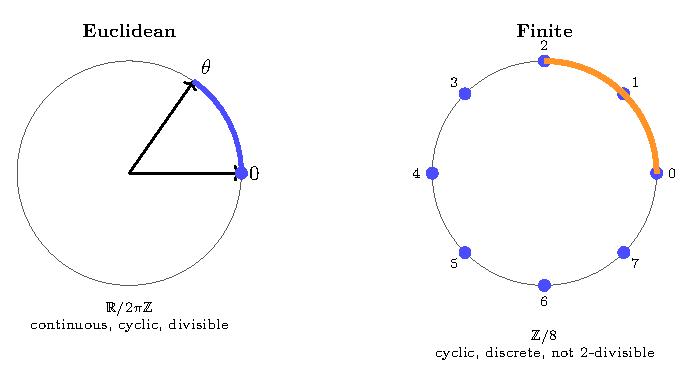
\includegraphics[width=0.86\textwidth]{finite-field-calculi/finite-trig/figures/fig-protractor.pdf}
\caption{The continuous protractor $\R/2\pi\Z$ and the finite protractor
$\Z/8$.  On the right the eight points of $C$ are the eight angles; the orange
arc $0\to2$ is the right angle, passing through the angle $1$.}
\label{fig:protractor}
\end{figure}

Table~\ref{tab:euclid-finite} records the group-algebraic properties, and
Table~\ref{tab:euclid-geometry} the order, continuity and line-based ones.

\begin{table}[htbp]
\centering
\small
\begin{tabularx}{\textwidth}{@{}>{\raggedright\arraybackslash}X>{\raggedright\arraybackslash}X>{\raggedright\arraybackslash}p{0.24\textwidth}@{}}
\toprule
Euclidean & finite unit-vector model & verdict\\
\midrule
angle group $\R/2\pi\Z$ & $\Z/8$ on $C$ & different cyclic groups\\
protractor additivity & $k+l\bmod 8$ & holds\\
right angle $\pi/2$; four right $=2\pi$ & $2$; $4\cdot2=8=0$ & holds\\
supplement/complement & $k+l=4$ / $k+l=2$ & holds\\
congruence is an equivalence & equality in $\Z/8$ & holds\\
angle copying & translation $k\mapsto k+h$ & holds\\
unique bisector & $2h=k$: $0$ or $2$ solutions & fails for odd $k$ (e.g.\ $k=1$)\\
$n$-section, all $n$ & $nh=k$ iff $\gcd(n,8)\mid k$ & fails in general\\
Thales (semicircle) & $(A-P)\cdot(B-P)=0$ & holds for $P\ne A,B$\\
inscribed angle $=$ half arc & $2h=\text{arc}$, $2$ not invertible & only $2$-to-$1$ here\\
\bottomrule
\end{tabularx}
\caption{Group-algebraic angle properties.  ``Holds'' means a definition and
proof; ``fails'' means a counterexample is given.  The inscribed-angle row is
the unit-vector reading; the line-direction reading is exact and appears below.}
\label{tab:euclid-finite}
\end{table}

\begin{table}[htbp]
\centering
\small
\begin{tabularx}{\textwidth}{@{}>{\raggedright\arraybackslash}X>{\raggedright\arraybackslash}X>{\raggedright\arraybackslash}p{0.26\textwidth}@{}}
\toprule
Euclidean & finite unit-vector model & verdict\\
\midrule
cyclic order & cyclic order & both; shared\\
compatible total order & none & neither has one\\
Archimedean & no order/continuity & Euclidean only\\
completeness & no order/continuity & Euclidean only\\
continuous measure & $\Z/8$-valued & no continuous measure\\
vertical angles equal & no angle between lines & not defined in this model\\
triangle angle sum $\pi$ & no angle at arbitrary vertices & not defined in this model; parallel postulate holds\\
similarity and AA & similarity group $\mathrm{GO}(Q)$ exists & AA not addressed\\
\bottomrule
\end{tabularx}
\caption{Order, continuity and line-based properties.  ``Not defined in this
model'' is not a counterexample; it means the unit-vector angle has no such
object.  The finite affine plane satisfies the parallel postulate.}
\label{tab:euclid-geometry}
\end{table}

\subsection{The line-direction model}

The unit-vector model is not the only finite angle; the line-direction ratio is
in the spirit of Wildberger's quadrance/spread \cite{Wildberger}.  Let
\[
  D=\F_{49}^\times/\F_7^\times .
\]
Since $|\F_{49}^\times|=48$ and $|\F_7^\times|=6$, $|D|=8$.  The map
\[
  \rho:D\longrightarrow G,\qquad \rho([z])=\frac z{\bar z},
\]
is an isomorphism: its kernel is $\F_7^\times$ (the condition $z=\bar z$), and
its image lies in the norm-one group $G$; both groups have order $8$.  A line
through the origin has a direction in $D$.  The eight points of $C$ map to four
lines (the antipodal pairs), while the other four directions have nonsquare
nonzero norm and contain no $\F_7$-point of $C$.  There are no nonzero
isotropic vectors over $\F_7$: $x^2+y^2=0$ would make $-1$ a square if
$y\ne0$, and if $y=0$ it also forces $x=0$.  For a direction represented by
$v$, a scalar multiple lies on $C$ exactly when $Q(v)$ is a nonzero square,
since $Q(cv)=c^2Q(v)$.

For distinct $A,B,P\in C$,
\begin{equation}\label{eq:line-inscribed}
  \boxed{\quad
  \rho\!\left(\frac{B-P}{A-P}\right)=\frac BA
  \quad}
\end{equation}
and the left side is independent of $P$.  The proof uses $\bar B=1/B$ and
$\bar P=1/P$:
\[
  \overline{B-P}=\bar B-\bar P=\frac1B-\frac1P
  =\frac{P-B}{BP}=-\frac{B-P}{BP},
\]
so
\[
  \rho\!\left(\frac{B-P}{A-P}\right)
  =\frac{(B-P)/(A-P)}{\overline{(B-P)/(A-P)}}
  =\frac{B-P}{A-P}\cdot\frac{\overline{A-P}}{\overline{B-P}}
  =\frac{B-P}{A-P}\cdot\frac{-(A-P)/(AP)}{-(B-P)/(BP)}
  =\frac{BP}{AP}=\frac BA .
\]
This is the exact line-direction inscribed-angle relation; it does not require
a half-angle in $\Z/8$.  It is checked for all $336$ ordered triples in
\texttt{verify.py}.

The line-direction angle between two lines with directions $d_1,d_2\in D$ is
$d_1/d_2\in G$.  Vertical angles are equal (the two pairs have the same ratio).
For a triangle with side directions $d_1,d_2,d_3$, the product of the three
turning ratios is $1$, so the oriented turning sum is $0$ (the full turn); this
is the exterior-angle statement, not the interior-angle sum $\pi$.  The
interior sum is a different statement and is not implied by the group law.

\begin{table}[htbp]
\centering
\small
\begin{tabular}{@{}lll@{}}
\toprule
 & unit-vector angle & line-direction angle\\
\midrule
values & $G=\Z/8$ & $D\cong G$\\
domain & points of $C$ & lines through $0$\\
coverage & $4$ lines ($8$ points) & all $8$ directions\\
inscribed angle & $2h=\text{arc}$ ($2$-to-$1$) & $\rho((B-P)/(A-P))=B/A$\\
vertical angles & not defined & equal\\
\bottomrule
\end{tabular}
\caption{The two finite angles.  The unit-vector angle is a point-on-conic
coordinate; the line-direction angle is a direction ratio.  Neither is a
failure of the other.}
\label{tab:angle-types}
\end{table}

\subsection{Three concrete comparisons}

\begin{example}[Bisection]\label{ex:bisection}
In Euclidean geometry every angle $0<\alpha<\pi$ has a unique bisector.  In the
unit-vector group $\Z/8$ the bisector equation is $2h=k$.  If $k$ is even there
are two solutions $h$ and $h+4$, the two orientations of the same bisector line;
the finite group has no total order with which to choose one.  If $k$ is odd there is
no solution.  For example, the right angle $k=2$ has $h=1,5$, while $k=1$ has no
bisector.  This is the failure of divisibility by $2$.
\end{example}

\begin{proposition}[Finite Thales]\label{prop:finite-thales}
Let $A,B\in C$ be antipodal, so $B=-A$, and let $P\in C$ with $P\ne A,B$.  Then
\[
  (A-P)\cdot(B-P)=A\cdot B-A\cdot P-P\cdot B+P\cdot P
  =-1-A\cdot P+A\cdot P+1=0 .
\]
Thus the vectors $PA$ and $PB$ are orthogonal with respect to the standard dot
product on $\F_7^2$: the angle in a semicircle is right, in the bilinear sense.
The algebraic identity also holds for $P=A$ or $P=B$, but then one of the
vectors $PA,PB$ is zero, so it is not an angle statement.
\end{proposition}

\begin{proof}
$A\cdot B=-1$ because $B=-A$ and $A\cdot A=1$; $P\cdot P=1$ because $P\in C$;
and $P\cdot B=P\cdot(-A)=-A\cdot P$.  The sum is zero.
\end{proof}

\begin{remark}[Triangle angle sum and inscribed angle]
The unit-vector model has no angle at an arbitrary vertex of a finite triangle:
the group $\Z/8$ is attached to the conic, not to arbitrary lines.  The
line-direction model does define the turning angles at a triangle; their
oriented sum is $0$ (the full turn), not the Euclidean interior sum $\pi$.  The
finite affine plane satisfies the parallel postulate, so the Euclidean triangle
angle sum is not a counterexample to it; the two statements are about different
angle structures.  Likewise, the unit-vector half-arc equation $2h=\text{arc}$
is only $2$-to-$1$, while the line-direction relation
\eqref{eq:line-inscribed} is exact and requires no halving.
\end{remark}

\subsection{What the comparison says}

The common algebraic skeleton is the angle group: a cyclic group acting
regularly on the circle or conic, with the angle as the group element.
Euclidean geometry adds an Archimedean continuous measure, completeness, and
divisibility.  It does \emph{not} add a compatible total order: neither the
Euclidean circle nor the finite one has one; both have a cyclic order.  The
finite affine plane also satisfies the parallel postulate.  The difference is
therefore continuity and divisibility, not total order and not the existence of
parallels.

The theorems that depend only on the group law survive: addition, supplements,
complements, right and straight angles, copying, and finite Thales.  The
theorems that need order, continuity, or division fail or are not defined:
bisection, $n$-section, the unit-vector triangle angle sum, and continuous
measure.  The line-direction model supplies an exact angle for arbitrary lines
and the exact inscribed relation \eqref{eq:line-inscribed}; the unit-vector
model supplies the point-on-conic coordinate.  This is the same pattern as the
$\R/\F_7$ trichotomy: the algebraic classification survives; the continuous
invariants do not.

\section{Stereographic and half-angle coordinates}
\label{sec:stereo}

\begin{figure}[htbp]
\centering
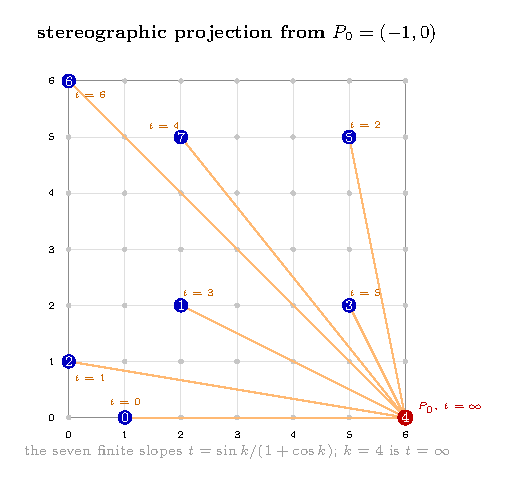
\includegraphics[width=0.52\textwidth]{finite-field-calculi/finite-trig/figures/fig-stereographic.pdf}
\caption{Stereographic projection from $P_0=(-1,0)=(6,0)$.  The seven finite
slopes $t=\sin k/(1+\cos k)$ give the seven points other than $P_0$; the point
$P_0$ itself is $t=\infty$.  The Euclidean segments are schematic: a projective
line over $\F_7$ contains eight points and wraps around the grid.}
\label{fig:stereo}
\end{figure}

For $k\ne4$ (so $\alpha^k\ne-1$), the line through $P_0=(-1,0)$ and
$(\cos k,\sin k)$ has slope
\begin{equation}\label{eq:t}
  t=\frac{\sin k}{1+\cos k}\in\F_7 .
\end{equation}
The inverse formulas are
\begin{equation}\label{eq:cos-sin-t}
  \cos k=\frac{1-t^2}{1+t^2},\qquad
  \sin k=\frac{2t}{1+t^2},
\end{equation}
and $k=4$ corresponds to $t=\infty$.  Thus
\[
  k\longmapsto t
\]
is a bijection $\Z/8\setminus\{4\}\to\F_7$, i.e.\ a finite half-angle
(tangent) coordinate.  The formulas \eqref{eq:t}--\eqref{eq:cos-sin-t} are
verified for all $k$ in \texttt{verify.py}.

\section{Discrete waveforms and the first difference}
\label{sec:waveforms}

\begin{figure}[htbp]
\centering
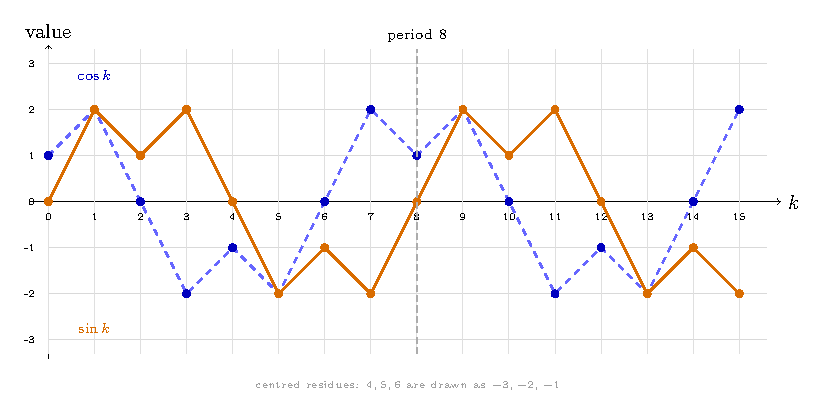
\includegraphics[width=0.86\textwidth]{finite-field-calculi/finite-trig/figures/fig-waveforms.pdf}
\caption{$\cos k$ and $\sin k$ as functions on $\Z/8$, repeated over two
periods.  The values are centred residues in $\{-3,\dots,3\}$; the dashed
vertical line marks the period $8$.  These are discrete waveforms, not
continuous graphs.}
\label{fig:waveforms}
\end{figure}

The functions $\cos$ and $\sin$ are periodic functions on the finite group
$\Z/8$.  Their first finite difference is
\[
  \Delta f(k)=f(k+1)-f(k).
\]
For example, with centred representatives,
\[
  \Delta\cos=(1,-2,-2,1,-1,2,2,-1),\qquad
  \Delta\sin=(2,-1,1,-2,-2,1,-1,2),
\]
and in both cases the sum over the cycle is $0$:
\[
  \sum_{k=0}^{7}\Delta f(k)=f(8)-f(0)=0 .
\]
This is the discrete fundamental theorem of calculus: summation and difference
are inverse up to the value at $0$.  Conversely, for $g:\Z/8\to\F_7$, the
equation $\Delta f=g$ has a solution if and only if
\[
  \sum_{k=0}^{7} g(k)=0 .
\]
The solutions are then $f+c$ for a constant $c$: the kernel of $\Delta$ is the
constants, and its image is the sum-zero functions.  This is the periodic
Fredholm alternative; it is the obstruction to a periodic antiderivative.

There is no limit, no derivative as a limit, and no mean value theorem; the
calculus here is finite and algebraic.  A caution about function spaces: a
polynomial \emph{function} on $\F_7$ is not the same object as a polynomial.
The polynomial $x^7-x$ vanishes at every point of $\F_7$, but its formal
derivative $7x^6-1=-1$ is not zero.  The derivation lives on polynomials and
rational functions, not on the algebra of $\F_7$-valued functions; to descend it
to point functions one must quotient by $x^7-x$, and the derivative does not
respect that quotient.  This is why the discrete calculus here is formal and
algebraic, not a calculus of arbitrary point functions.

The next section gives the finite-field Fourier layer.  A systematic treatment
of $\Delta$, summation, Hasse derivatives and residues on
$\mathbb P^1(\F_7)$ is the next note.

\section{The harmonic layers}
\label{sec:fourier}

The algebraic trigonometry of the previous sections takes values in $\F_7$.
There are two harmonic layers above it, and they must not be conflated: a
finite-field layer with values in $\F_{49}$, and a complex layer with values in
$\C$.  The first is the algebraic bridge; the second is a unitary
representation.

\subsection{The finite-field layer}

Let
\[
  \chi_j(k)=\alpha^{jk}\in\F_{49},\qquad j,k\in\Z/8 .
\]
These are the finite-field characters of $\Z/8$.  Orthogonality reads
\[
  \sum_{k=0}^{7}\chi_j(k)\chi_{-l}(k)=8\,\delta_{jl}.
\]
The field $\F_{49}$ has characteristic $7$, so $8=1\ne0$; the sum is $1$ for
$j=l$ and $0$ otherwise.  For a function $f:\Z/8\to\F_{49}$ define
\[
  \widehat f(j)=\sum_{k=0}^{7} f(k)\chi_{-j}(k),
  \qquad
  f(k)=8^{-1}\sum_{j=0}^{7}\widehat f(j)\chi_j(k),
\]
with $8^{-1}=1$.  The Fourier matrix $(\chi_j(k))_{j,k}$ is invertible; the
transform is an isomorphism of the $8$-dimensional space of functions.

The difference operator acts on the characters by
\[
  \Delta\chi_j=(\alpha^j-1)\chi_j .
\]
Thus the characters are the eigenvectors of $\Delta$, with eigenvalues
$\alpha^j-1$.  The eigenvalues are distinct because $\alpha^j$ are distinct;
the Fourier transform diagonalizes $\Delta$.  The constants are $j=0$ with
eigenvalue $0$, and the image of $\Delta$ is the sum-zero functions, in
agreement with the solvability condition of \S\ref{sec:waveforms}.

The trigonometric functions are the real and imaginary coordinates in this
basis:
\[
  \cos k=\frac{\chi_1(k)+\chi_{-1}(k)}2,
  \qquad
  \sin k=\frac{\chi_1(k)-\chi_{-1}(k)}{2\ii}.
\]
Their Fourier transforms have support on $j=\pm1$.  In this sense the
finite-field Fourier layer is the algebraic bridge between the $\cos/\sin$
tables and the difference operator: the same $\alpha$ produces the point
coordinates, the characters, and the spectrum.

\subsection{The complex layer}

\begin{figure}[htbp]
\centering
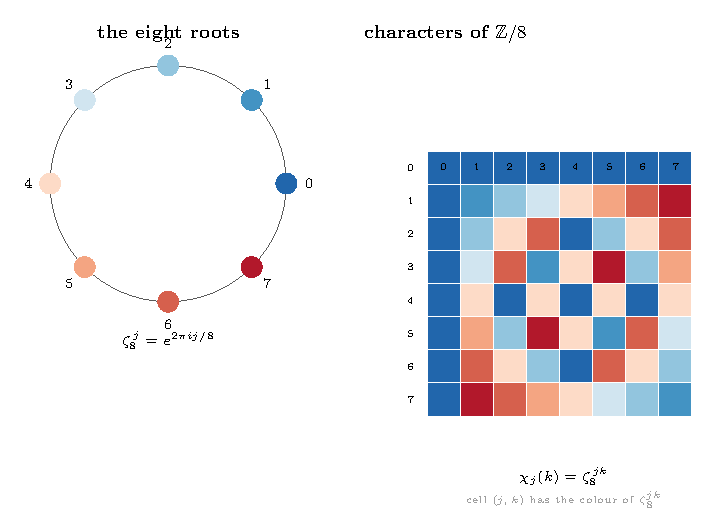
\includegraphics[width=0.86\textwidth]{finite-field-calculi/finite-trig/figures/fig-fourier.pdf}
\caption{The complex harmonic layer.  Left: the eight eighth roots of unity
$\zeta_8^j$.  Right: the character matrix $\chi_j(k)=\zeta_8^{jk}$; the cell
$(j,k)$ has the colour of $\zeta_8^{jk}$.}
\label{fig:fourier}
\end{figure}

A second harmonic layer takes values in $\C$.  Let
\[
  \zeta_8=e^{2\pi\ii/8}
\]
and define the complex characters of $\Z/8$ by
\[
  \chi_j(k)=\zeta_8^{jk},\qquad j,k\in\Z/8 .
\]
For a function $f:\Z/8\to\C$, the finite Fourier transform is
\[
  \widehat f(j)=\sum_{k=0}^{7} f(k)\,\zeta_8^{-jk},
\]
with inversion
\[
  f(k)=\frac18\sum_{j=0}^{7}\widehat f(j)\,\zeta_8^{jk}
\]
and Parseval
\[
  \sum_{k=0}^{7}|f(k)|^2=\frac18\sum_{j=0}^{7}|\widehat f(j)|^2 .
\]
The transform diagonalizes translations: if $(\tau_a f)(k)=f(k-a)$, then
$\widehat{\tau_a f}(j)=\zeta_8^{-ja}\widehat f(j)$.  For the general theory of
Fourier analysis on finite groups see \cite{FTN}.

\subsection{The two layers}

The finite-field characters $\chi_j^{\F}(k)=\alpha^{jk}\in\F_{49}$ and the
complex characters $\chi_j^{\C}(k)=\zeta_8^{jk}\in\C$ share the index group
$\Z/8$ and the same orthogonality pattern, but they take values in different
fields.  The finite-field layer is algebraic: it diagonalizes $\Delta$, and the
$\cos/\sin$ coordinates are its $\pm1$ modes.  The complex layer is unitary: it
gives the Hilbert-space transform and Parseval.  Neither is a substitute for the
other.

The bridge between the additive characters of $\F_7$ and the multiplicative
characters of $\F_7^\times$ is the Gauss sum
\[
  G(\chi)=\sum_{x\in\F_7}\chi(x)\,\zeta_7^{x},
\]
which is the finite analogue of the Gamma integral; it will be treated in the
next note.  A further bridge between finite point functions, rational functions
on $\mathbb P^1(\F_7)$, and functions on local fields is the subject of the
discrete-calculus note; the polynomial $x^7-x$ of \S\ref{sec:waveforms} is the
basic warning that these are different function spaces.

\section{What is not claimed, and what comes next}
\label{sec:boundary}

This note is deliberately small.  It does \emph{not} claim:
\begin{itemize}
  \item a real or complex analysis over $\F_7$: there are no nontrivial limits,
        no continuity in the analytic sense, no mean value theorem;
  \item that the finite trigonometry is a picture of the real one: the values
        are in $\F_7$, the angle group is $\Z/8$, and the identities are
        algebraic;
  \item that the conic or Pascal's theorem alone gives analysis: the conic gives
        the geometry and the group law; the analysis comes from the derivation,
        difference, representation and cohomological structures built on top;
  \item that the finite-field Fourier layer and the complex Fourier layer are
        the same representation: they share the index group but take values in
        different fields.
\end{itemize}

The finite-field Fourier layer of Section~\ref{sec:fourier} is now included.
The next installment, \emph{Conic Motions, Arithmetic Histories, and Three
Finite Calculi} (\href{49-conic-histories-and-finite-calculi.pdf}{companion note 49}), now gives the
arithmetic-history realization of the eight-point circle step, its ordinary
evaluation domains, and the comparison with split six-cycles and unipotent
seven-cycles.  In characteristic seven the last has a nilpotent difference,
whereas the first two admit Fourier diagonalization over appropriate fields.
Further directions after this history/calculus interface are:
\begin{enumerate}
  \item discrete calculus on $\mathbb P^1(\F_7)$: $\Delta$, summation, Hasse
        derivatives, differential forms, residues and the residue theorem,
        together with the function-space distinctions (the polynomial
        $x^7-x$ versus the function it defines);
  \item Gauss sums and the bridge between the additive and multiplicative
        characters;
  \item the harmonic analysis of functions on $\mathrm{PGL}_2(\F_7)$ and the
        Bruhat--Tits tree \cite{Serre}, as a non-Archimedean analogue of the
        hyperbolic analysis of Paper~\cite{Paper0}/Paper~\cite{Paper1};
  \item the characteristic-$7$ Magnus expansion and the group algebra
        $\F_7[\mathrm{PGL}_2(\F_7)]$, as the finite analogue of the series
        pillar of Paper~\cite{Paper1}.
\end{enumerate}

\paragraph{Scope.}
Sections~1--4 and 7--10 form the trigonometry and difference core;
Sections~5--6 (transformations, centres, arcs, ripple) are a geometric
excursion.  They can be split into a second paper once the foundations settle;
the present revision keeps them together so that the cross-references remain
explicit.

\begin{thebibliography}{99}
\bibitem{Serre} J.-P.~Serre, \emph{Trees}, Springer, 1980.
\bibitem{FTN} A.~Terras, \emph{Fourier Analysis on Finite Groups and
Applications}, Cambridge University Press, 1999.
\bibitem{Lidl} R.~Lidl and H.~Niederreiter, \emph{Finite Fields},
Cambridge University Press, 1997.
\bibitem{FFTrig} M.~Saaltink, \emph{Generalized trigonometry and Chebyshev
functions in finite fields}, Finite Fields Appl. \textbf{86} (2023), 102143,
\url{https://doi.org/10.1016/j.ffa.2022.102143}.
\bibitem{Wildberger} N.~J.~Wildberger, \emph{The ancient Greeks present:
Rational trigonometry}, arXiv:0806.3481 (2008),
\url{https://arxiv.org/abs/0806.3481}.
\bibitem{Paper0} M.~Yuan, \emph{Arithmetic Expression Geometry 0: Arithmetic
Expression Spaces}, 2026, \url{https://github.com/mountain/aeg-paper}.
\bibitem{Paper1} M.~Yuan, \emph{Arithmetic Expression Geometry I: Foundations},
2026, \url{https://github.com/mountain/aeg-paper}.
\end{thebibliography}

\end{document}
